
本章的其余部分中,我们将更详细地了解每种性能分析工具。本节中,我们将做一个端到端示例,并分析程序的性能。这将展示如何进行性能分析,以及如何使用不同的性能分析工具。

本节结束时,读者们应该会相信“永远不要对性能进行猜测”。

实际中需要分析和优化的实际程序很可能大到要用很多页来说明,因此我们将使用一个简化的示例。程序中将完成对子字符串的排序:假设有一个字符串\texttt{S},比如:“\texttt{abcdcba}”(这里是个简单的例子,实际的字符串将有数百万字符)。可以从该字符串中的任何字符开始创建子字符串,例如:\texttt{S0}的起始偏移量为0,因此其值为“\texttt{abcdcba}”。\texttt{S2}以偏移量2开始,值为“\texttt{cdcba}”,S5为“\texttt{ba}”。我们要用常规的字符串比较来按顺序对这些子字符串进行排序,子字符串的顺序是\texttt{S2},\texttt{S5},\texttt{S0}(按照第一个字符\texttt{'c'}、\texttt{'b'}和\texttt{'a'}的顺序)。

如果用字符指针表示子字符串,就可以使用STL排序算法\texttt{std::sort}进行排序:现在交换两个子字符串只需要交换指针,而底层字符串保持不变。下面是示例代码:

\hspace*{\fill} \\ %插入空行
\noindent
\textbf{01\_substring\_sort.C}
\begin{lstlisting}[style=styleCXX]
bool compare(const char* s1, const char* s2, unsigned int l);
int main() {
	constexpr unsigned int L = …, N = …;
	unique_ptr<char[]> s(new char[L]);
	vector<const char*> vs(N);
	  … prepare the string …
	size_t count = 0;
	system_clock::time_point t1 = system_clock::now();
	std::sort(vs.begin(), vs.end(),
	  [&](const char* a, const char* b) {
		++count;
		return compare(a, b, L);
	});
	system_clock::time_point t2 = system_clock::now();
	cout << "Sort time: " <<
	  duration_cast<milliseconds>(t2 - t1).count() <<
	  "ms (" << count << " comparisons)" << endl;
}
\end{lstlisting}

注意,为了编译这个例子,需要包含相应的头文件,并为名字缩短使用\texttt{using}声明:

\begin{lstlisting}[style=styleCXX]
#include <algorithm>
#include <chrono>
#include <cstdlib>
#include <cstring>
#include <iostream>
#include <memory>
#include <random>
#include <vector>
using std::chrono::duration_cast;
using std::chrono::milliseconds;
using std::chrono::system_clock;
using std::cout;
using std::endl;
using std::minstd_rand;
using std::unique_ptr;
using std::vector;
\end{lstlisting}

后面的例子中,我们将省略公共头文件和公共名称(如\texttt{cout}或\texttt{vector})的\texttt{using}声明。

示例定义了一个字符串,该字符串用于要排序的子字符串和子字符串组(字符指针)的底层数据(但这里还没有展示数据本身是如何创建的)。然后,使用\texttt{std::sort}和比较函数对子字符串进行排序:一个调用比较函数compare()的lambda表达式。我们使用lambda表达式将compare()函数的输入(该函数接受两个指针和最大字符串长度)调整为\texttt{std::sort}所期望的输入(只有两个指针)。这就是适配器模式。

我们的例子中,lambda表达式的第二个作用:计算比较调用的次数。因为我们对排序的性能很感兴趣,所以如果想比较不同的排序算法,这个信息可能会很有用(我们现在不打算这么做,但是这个技术可能对读者们的性能优化工作很有用)。

这个例子中只声明了比较函数,但没有定义。它的定义在一个单独的文件中,如下所示:


\hspace*{\fill} \\ %插入空行
\noindent
\textbf{01\_substring\_sort\_a.C}
\begin{lstlisting}[style=styleCXX]
bool compare(const char* s1, const char* s2, unsigned int l) {
	if (s1 == s2) return false;
	for (unsigned int i1 = 0, i2 = 0; i1 < l; ++i1, ++i2) {
		if (s1[i1] != s2[i2]) return s1[i1] > s2[i2];
	}
	return false;
}
\end{lstlisting}

比较两个字符串的简单比较:如果第一个字符串大于第二个字符串,则返回true,否则返回false。我们可以将函数定义在与代码本身相同的文件中,但即是这个小示例,我们也尝试模拟真实程序的行为,该程序可能会使用分布在许多不同文件中的函数。因此,本章的\texttt{compare.C}文件中的实现了比较函数,其余的例子在\texttt{example.C}文件中。

最后,我们使用\texttt{chrono}库中的高精度计时器来测量,进行子字符串排序所需的时间。

在我们的示例中缺少字符串的实际数据。子字符串排序在许多应用程序中是一项常见的任务,并且每个应用程序都有自己的获取数据的方法。我们的例子中,可以使用生成的随机字符串。另一方面,许多子字符串排序的实际应用,会有一个字符在字符串中出现的频率比其他任何字符都要高。

我们也可以模拟这种类型的数据,用一个字符填充字符串,然后随机改变其中的一些:

\hspace*{\fill} \\ %插入空行
\noindent
\textbf{01\_substring\_sort\_a.C}
\begin{lstlisting}[style=styleCXX]
constexpr unsigned int L = 1 << 18, N = 1 << 14;
unique_ptr<char[]> s(new char[L]);
vector<const char*> vs(N);
minstd_rand rgen;
::memset(s.get(), 'a', N*sizeof(char));
for (unsigned int i = 0; i < L/1024; ++i) {
	s[rgen() % (L - 1)] = 'a' + (rgen() % ('z' - 'a' + 1));
}
s[L-1] = 0;
for (unsigned int i = 0; i < N; ++i) {
	vs[i] = &s[rgen() % (L - 1)];
}
\end{lstlisting}

字符串的长度\texttt{L}和子字符串的数量\texttt{N}是适配相应机器上的运行时长,从而用来运行这些测试的(如果想在其他设备上重复运行这个例子,可能需要调整相应的数字,运行速度速度取决于使用的处理器)。

现在我们的例子已经可以编译和运行了:

%\hspace*{\fill} \\ %插入空行
\begin{center}
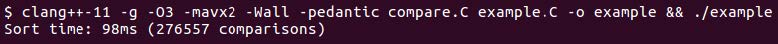
\includegraphics[width=0.9\textwidth]{content/1/chapter2/images/1.jpg}\\
图 2.1
\end{center}

得到的结果取决于您使用的编译器、运行的计算机。当然,还取决于数据语料库。

现在我们有了第一个性能测试。你可能会问的第一个问题是,我们如何优化它?这并不是你应该问的第一个问题。第一个问题应该是,我们需要优化吗?要回答这个问题,需要有性能的目标和指标,以及这个项目其他部分的相对性能的数据,例如:如果实际的字符串是由一个耗时10小时的模拟生成的,那么排序所花费的100秒的时间几乎不值一提。当然,我们仍然在处理模拟示例,除非我们必须要提高性能,否则本章不会对优化进行深入的讨论。

我们准备好讨论如何优化它了吗?这个问题先等等,现在的问题应该是,\textbf{我们应该优化什么}?或者说,程序在什么地方花费的时间最多?即使在这个例子中,这个耗时热点也可能是排序或比较函数。我们不能访问这种类型的源代码(除非我们想破坏标准库),但是可以将计时器放入到比较函数中。

不过,这不太可能产生好的结果:如果每次运行比较都非常快,因为调用计时器也需要时间,所以每次调用比较函数时,调用计时器的时间将对我们的测试结果有比较大的影响。实际的程序中,这种带有计时器的结构几乎没有。如果不知道时间耗费在哪里,就需要在数百个函数中安插计时器(如果没有任何测试,要如何知道这一点?)。所以,这时就需要性能分析工具来帮助我们来完成一些工作了。

下一节中了解更多关于分析器的知识。现在,只需了解以下命令行将编译和执行的程序,并使用GperfTools包中的谷歌分析器收集其运行时的相关信息:

%\hspace*{\fill} \\ %插入空行
\begin{center}
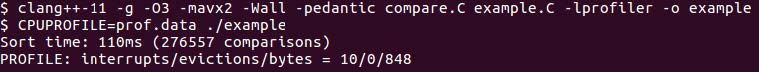
\includegraphics[width=0.9\textwidth]{content/1/chapter2/images/2.jpg}\\
图 2.2
\end{center}

数据放在\texttt{prof.data}文件中,其路径由\texttt{CPUPROFILE}环境变量指定。细心的读者可能已经注意到,这次程序运行的时间更长了,这是性能分析几乎不可避免的副作用。假设分析器本身工作正常,那么程序不同部分的相对性能仍然是准确的。

输出的最后一行说明,分析器已经收集了一些数据,现在我们需要以可读的格式显示这些数据。对于谷歌分析器收集的数据,用户界面工具是\texttt{google-pprof}(通常安装为简单的\texttt{pprof}),最简单的方式是列出程序中的每个函数,以及在该函数中花费时间的百分比(第二列):

%\hspace*{\fill} \\ %插入空行
\begin{center}
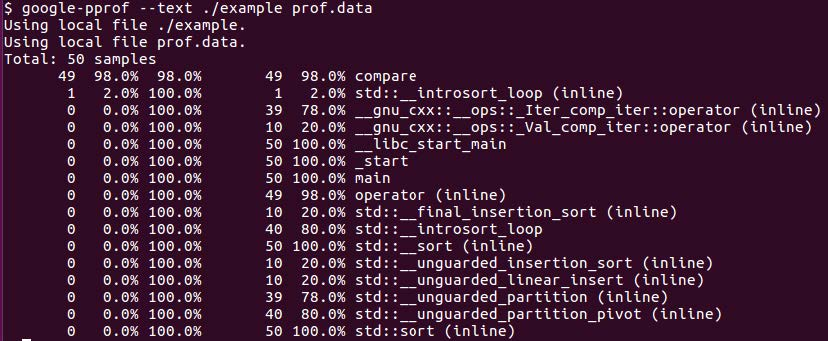
\includegraphics[width=0.9\textwidth]{content/1/chapter2/images/3.jpg}\\
图 2.3
\end{center}

分析器显示,几乎所有的时间都花在比较函数\texttt{compare()}上,而排序几乎不花任何时间(第二行是\texttt{std::sort},应该认为是排序所花时间的一部分)。请注意,对于任何分析,都需要收集50个以上的样本数据。样本数据的数量取决于程序运行的时间,为了获得可靠的数据,需要在每个要测试的函数中积累至少几十个样本数据。就我们的情况而言,其结果比较容易判断,因此我们会按我们收集的数据来做分析。

由于子字符串比较函数占用了总运行时间的98\%,我们只有两种方法来提高性能:可以使这个函数更快,或者可以减少使用次数(许多人忘记了第二种可能性,直接使用第一种可能性)。第二种方法需要使用不同的排序算法,不在本书的讨论范围之内。这里我们将重点讨论第一个选项。让我们再来看一下比较函数的代码:

\hspace*{\fill} \\ %插入空行
\noindent
\textbf{01\_substring\_sort\_a.C}
\begin{lstlisting}[style=styleCXX]
bool compare(const char* s1, const char* s2, unsigned int l) {
	if (s1 == s2) return false;
	for (unsigned int i1 = 0, i2 = 0; i1 < l; ++i1, ++i2) {
		if (s1[i1] != s2[i2]) return s1[i1] > s2[i2];
	}
	return false;
}
\end{lstlisting}

这只是几行代码,我们应该能够理解和预测代码的所有行为。还有一个比较子字符串和它本身的检查,这肯定比实际逐字符进行比较要快,所以,除非我们确定函数调用时两个指针的值不会相同,否则这一行肯定保持不变。

还有一个循环(循环的主体是一次比较一个字符),这里必须这样做,因为我们不知道哪个字符可能不同。循环本身会一直运行,直到找到一个差值或比较最大可能的字符数为止。显而易见,后一种情况是不可能发生的:该字符串以空字符结尾,即使两个子字符串中的所有字符都相同,我们迟早会到达较短子字符串的末尾,将其末尾的空字符与另一个子字符串中的非空字符进行比较,从而确定较短的子字符串是两者中较短的字符串。

只有当两个子字符串都从同一个位置开始时,我们才有可能读取字符串末尾以外的内容,所以我们在函数的一开始就进行了检查。这很好!我们发现了一些不必要的工作,因此可以优化代码,并避免每次循环迭代都进行一次比较操作(考虑到循环体中没有很多其他操作,这应该是非常重要的)。

代码中的改动非常简单:只需删除循环对长度的比较操作(我们也不再需要将长度传递给比较函数):

\hspace*{\fill} \\ %插入空行
\noindent
\textbf{03\_substring\_sort\_a.C}
\begin{lstlisting}[style=styleCXX]
bool compare(const char* s1, const char* s2) {
	if (s1 == s2) return false;
	for (unsigned int i1 = 0, i2 = 0;; ++i1, ++i2) {
		if (s1[i1] != s2[i2]) return s1[i1] > s2[i2];
	}
	return false;
}
\end{lstlisting}

更少的参数,更少的操作,更少的代码。让我们运行这个程序,看看这次优化为节省了多少运行时间:

%\hspace*{\fill} \\ %插入空行
\begin{center}
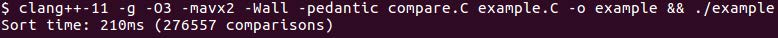
\includegraphics[width=0.9\textwidth]{content/1/chapter2/images/4.jpg}\\
图 2.4
\end{center}

如果说事情没有按计划进行,那就太保守了。原来的代码花了98毫秒来解决相同的问题(图2.1)。“优化后的”代码需要210毫秒,尽管做的工作更少(注意,在这个例子中,并不是所有的编译器都表现出这种特殊的性能异常,但我们使用的是生产过程中使用的编译器。这里没有欺骗,这种情况也可能发生在你身上)。

总结一下这个例子,它实际上是一个现实程序的浓缩。当我们试图优化这段代码时,另一个开发者正在使用代码的另一部分,并且还需要一个子字符串比较函数。将单独开发的代码片段放在一起,只保留了这个函数的一个版本,而它恰好是我们没有修改的那个;其他开发者的修改几乎同样:

\hspace*{\fill} \\ %插入空行
\noindent
\textbf{04\_substring\_sort\_a.C}
\begin{lstlisting}[style=styleCXX]
bool compare(const char* s1, const char* s2) {
	if (s1 == s2) return false;
	for (int i1 = 0, i2 = 0;; ++i1, ++i2) {
		if (s1[i1] != s2[i2]) return s1[i1] > s2[i2];
	}
	return false;
}
\end{lstlisting}

仔细关闸这段代码和它前面的代码片段,看看是否能发现区别。

唯一的区别是循环变量的类型:之前,我们使用了\texttt{unsigned int},索引从0开始并向前推进,我们不期望有任何负数。最后一个代码片段使用了\texttt{int},放弃了可能的索引值范围的一半。

对于这个代码的修改,我们可以再次运行我们的基准测试,这次是用新的比较函数。结果还是出人意料:

%\hspace*{\fill} \\ %插入空行
\begin{center}
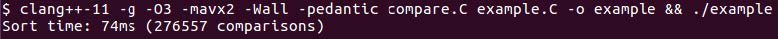
\includegraphics[width=0.9\textwidth]{content/1/chapter2/images/5.jpg}\\
图 2.5
\end{center}

最新版本耗时74毫秒,比我们最初的版本(98毫秒,图2.1)快,也比几乎相同的第二个版本(210毫秒,图2.2)快得多。

下一章我们再来解释这个现象的原因。本节的目的是阐明\textbf{永远不要猜测性能}:“显而易见”的优化——用更少的代码做完全相同的计算——引人注目地反向进行,而本不重要的小改变——使用有符号整数而不是无符号的函数,无论如何所有值都是非负的——结果证明是一个有效的优化。

即使在这个非常简单的例子中,性能结果也可能与直觉相反。因此,对于性能的良好决策的唯一方法必须是指标驱动。本章的其余部分,我们将看到一些最常用的工具,用于收集性能指标,学习如何使用它们,以及如何解释其结果。
